\begin{figure}[htb]
\centering
\subfloat[$\fancy{N}_1$]{\label{fig:neighborhood1}
\begin{tikzpicture}[scale = 10]
\tikzstyle{VertexStyle}=[shape = circle,	
								 minimum size = 1pt,
								 inner sep = 1.2pt,
                         draw]
\Vertex[x = 0.161400005221367, y = 0.859399989247322, L = \tiny {$v_3$}]{v0}
\Vertex[x = 0.250200033187866, y = 0.85819998383522, L = \tiny {$v_4$}]{v1}
\Vertex[x = 0.160599991679192, y = 0.939399991184473, L = \tiny {$v_1$}]{v2}
\Vertex[x = 0.249400034546852, y = 0.938199985772371, L = \tiny {$v_2$}]{v3}
\Vertex[x = 0.16219998896122, y = 0.780199974775314, L = \tiny {$v_5$}]{v4}
\Vertex[x = 0.250999987125397, y = 0.778999969363213, L = \tiny {$v_6$}]{v5}
\Edge[](v1)(v0)
\Edge[](v3)(v2)
\Edge[](v1)(v3)
\Edge[](v0)(v2)
\Edge[](v5)(v4)
\Edge[](v5)(v1)
\Edge[](v4)(v0)
\end{tikzpicture}
}\qquad\qquad
\subfloat[$\fancy{N}_2$]{\label{fig:neighborhood2}
\begin{tikzpicture}[scale = 10]
\tikzstyle{VertexStyle}=[shape = circle,	
								 minimum size = 1pt,
								 inner sep = 1.2pt,
                         draw]
\Vertex[x = 0.161400005221367, y = 0.859399989247322, L = \tiny {$v_3$}]{v0}
\Vertex[x = 0.250200033187866, y = 0.85819998383522, L = \tiny {$v_4$}]{v1}
\Vertex[x = 0.160599991679192, y = 0.939399991184473, L = \tiny {$v_1$}]{v2}
\Vertex[x = 0.249400034546852, y = 0.938199985772371, L = \tiny {$v_2$}]{v3}
\Vertex[x = 0.16219998896122, y = 0.780199974775314, L = \tiny {$v_5$}]{v4}
\Vertex[x = 0.250999987125397, y = 0.778999969363213, L = \tiny {$v_6$}]{v5}
\Edge[](v1)(v0)
\Edge[](v3)(v2)
\Edge[](v1)(v3)
\Edge[](v0)(v2)
\Edge[](v5)(v4)
\Edge[](v5)(v1)
\Edge[](v4)(v0)
\Edge[](v2)(v1)
\end{tikzpicture}
}\qquad\qquad
\subfloat[$\fancy{N}_3$]{\label{fig:neighborhood3}
\begin{tikzpicture}[scale = 10]
\tikzstyle{VertexStyle}=[shape = circle,	
								 minimum size = 1pt,
								 inner sep = 1.2pt,
                         draw]
\Vertex[x = 0.161400005221367, y = 0.859399989247322, L = \tiny {$v_3$}]{v0}
\Vertex[x = 0.250200033187866, y = 0.85819998383522, L = \tiny {$v_4$}]{v1}
\Vertex[x = 0.160599991679192, y = 0.939399991184473, L = \tiny {$v_1$}]{v2}
\Vertex[x = 0.250200033187866, y = 0.938999984413385, L = \tiny {$v_2$}]{v3}
\Vertex[x = 0.16219998896122, y = 0.780199974775314, L = \tiny {$v_5$}]{v4}
\Vertex[x = 0.250999987125397, y = 0.778999969363213, L = \tiny {$v_6$}]{v5}
\Edge[](v1)(v0)
\Edge[](v3)(v2)
\Edge[](v0)(v2)
\Edge[](v5)(v4)
\Edge[](v5)(v1)
\Edge[](v4)(v0)
\Edge[](v2)(v1)
\Edge[style = {bend left}](v3)(v5)
\end{tikzpicture}
}\qquad\qquad
\subfloat[$\fancy{N}_4$]{\label{fig:neighborhood4}
\begin{tikzpicture}[scale = 10]
\tikzstyle{VertexStyle}=[shape = circle,	
								 minimum size = 1pt,
								 inner sep = 1.2pt,
                         draw]
\Vertex[x = 0.161400005221367, y = 0.859399989247322, L = \tiny {$v_3$}]{v0}
\Vertex[x = 0.250200033187866, y = 0.85819998383522, L = \tiny {$v_4$}]{v1}
\Vertex[x = 0.160599991679192, y = 0.939399991184473, L = \tiny {$v_1$}]{v2}
\Vertex[x = 0.251000016927719, y = 0.941399987787008, L = \tiny {$v_2$}]{v3}
\Vertex[x = 0.16219998896122, y = 0.780199974775314, L = \tiny {$v_5$}]{v4}
\Vertex[x = 0.250999987125397, y = 0.778999969363213, L = \tiny {$v_6$}]{v5}
\Edge[](v1)(v0)
\Edge[](v3)(v2)
\Edge[](v1)(v3)
\Edge[](v0)(v2)
\Edge[](v5)(v4)
\Edge[](v5)(v1)
\Edge[](v4)(v0)
\Edge[](v2)(v1)
\Edge[style = {bend left}](v3)(v5)
\end{tikzpicture}
}\qquad\qquad
\subfloat[$\fancy{N}_5$]{\label{fig:neighborhood5}
\begin{tikzpicture}[scale = 10]
\tikzstyle{VertexStyle}=[shape = circle,	
								 minimum size = 1pt,
								 inner sep = 1.2pt,
                         draw]
\Vertex[x = 0.161400005221367, y = 0.859399989247322, L = \tiny {$v_3$}]{v0}
\Vertex[x = 0.250200033187866, y = 0.85819998383522, L = \tiny {$v_4$}]{v1}
\Vertex[x = 0.160599991679192, y = 0.939399991184473, L = \tiny {$v_1$}]{v2}
\Vertex[x = 0.250200033187866, y = 0.938999984413385, L = \tiny {$v_2$}]{v3}
\Vertex[x = 0.16219998896122, y = 0.780199974775314, L = \tiny {$v_5$}]{v4}
\Vertex[x = 0.250999987125397, y = 0.778999969363213, L = \tiny {$v_6$}]{v5}
\Edge[](v1)(v0)
\Edge[](v3)(v2)
\Edge[](v0)(v2)
\Edge[](v5)(v4)
\Edge[](v5)(v1)
\Edge[](v4)(v0)
\Edge[style = {bend left}](v3)(v5)
\end{tikzpicture}
}\qquad\qquad
\subfloat[$\fancy{N}_6$]{\label{fig:neighborhood6}
\begin{tikzpicture}[scale = 10]
\tikzstyle{VertexStyle}=[shape = circle,	
								 minimum size = 1pt,
								 inner sep = 1.2pt,
                         draw]
\Vertex[x = 0.0898210406303406, y = 0.898352794349194, L = \tiny {$v_3$}]{v0}
\Vertex[x = 0.178257435560226, y = 0.898970954120159, L = \tiny {$v_4$}]{v1}
\Vertex[x = 0.133311897516251, y = 0.95333456993103, L = \tiny {$v_1$}]{v2}
\Vertex[x = 0.133166402578354, y = 0.859043657779694, L = \tiny {$v_2$}]{v3}
\Vertex[x = 0.09025739133358, y = 0.819152742624283, L = \tiny {$v_5$}]{v4}
\Vertex[x = 0.179057389497757, y = 0.818680047988892, L = \tiny {$v_6$}]{v5}
\Vertex[x = 0.224584609270096, y = 0.85951641201973, L = \tiny {$v_7$}]{v6}
\Edge[](v1)(v0)
\Edge[](v0)(v2)
\Edge[](v5)(v4)
\Edge[](v5)(v1)
\Edge[](v4)(v0)
\Edge[](v2)(v1)
\Edge[](v3)(v0)
\Edge[](v3)(v1)
\Edge[](v6)(v1)
\Edge[](v6)(v5)
\end{tikzpicture}
}\qquad\qquad
\subfloat[$\fancy{N}_7$]{\label{fig:neighborhood7}
\begin{tikzpicture}[scale = 10]
\tikzstyle{VertexStyle}=[shape = circle,	
								 minimum size = 1pt,
								 inner sep = 1.2pt,
                         draw]
\Vertex[x = 0.193747192621231, y = 0.853734999895096, L = \tiny {$v_3$}]{v0}
\Vertex[x = 0.282183587551117, y = 0.854353159666061, L = \tiny {$v_4$}]{v1}
\Vertex[x = 0.237238049507141, y = 0.908716790378094, L = \tiny {$v_1$}]{v2}
\Vertex[x = 0.237092554569244, y = 0.814425885677338, L = \tiny {$v_2$}]{v3}
\Vertex[x = 0.194183543324471, y = 0.774534970521927, L = \tiny {$v_5$}]{v4}
\Vertex[x = 0.282983541488647, y = 0.774062275886536, L = \tiny {$v_6$}]{v5}
\Vertex[x = 0.237433806061745, y = 0.971821719780564, L = \tiny {$v_7$}]{v6}
\Edge[](v1)(v0)
\Edge[](v0)(v2)
\Edge[](v5)(v4)
\Edge[](v5)(v1)
\Edge[](v4)(v0)
\Edge[](v2)(v1)
\Edge[](v3)(v0)
\Edge[](v3)(v1)
\Edge[style = {bend right}](v6)(v0)
\Edge[style = {bend left}](v6)(v1)
\end{tikzpicture}
}\qquad\qquad
\subfloat[$\fancy{N}_8$]{\label{fig:neighborhood8}
\begin{tikzpicture}[scale = 10]
\tikzstyle{VertexStyle}=[shape = circle,	
								 minimum size = 1pt,
								 inner sep = 1.2pt,
                         draw]
\Vertex[x = 0.193747192621231, y = 0.853734999895096, L = \tiny {$v_3$}]{v0}
\Vertex[x = 0.282183587551117, y = 0.854353159666061, L = \tiny {$v_4$}]{v1}
\Vertex[x = 0.237238049507141, y = 0.908716790378094, L = \tiny {$v_1$}]{v2}
\Vertex[x = 0.237092554569244, y = 0.814425885677338, L = \tiny {$v_2$}]{v3}
\Vertex[x = 0.194183543324471, y = 0.774534970521927, L = \tiny {$v_5$}]{v4}
\Vertex[x = 0.282983541488647, y = 0.774062275886536, L = \tiny {$v_6$}]{v5}
\Vertex[x = 0.237433806061745, y = 0.971821719780564, L = \tiny {$v_7$}]{v6}
\Edge[](v1)(v0)
\Edge[](v0)(v2)
\Edge[](v5)(v4)
\Edge[](v5)(v1)
\Edge[](v4)(v0)
\Edge[](v2)(v1)
\Edge[](v3)(v0)
\Edge[](v3)(v1)
\Edge[style = {bend right}](v6)(v0)
\Edge[style = {bend left}](v6)(v1)
\Edge[](v6)(v2)
\Edge[](v2)(v3)
\end{tikzpicture}
}\qquad\qquad
\subfloat[$\fancy{N}_9$]{\label{fig:neighborhood9}
\begin{tikzpicture}[scale = 10]
\tikzstyle{VertexStyle}=[shape = circle,	
								 minimum size = 1pt,
								 inner sep = 1.2pt,
                         draw]
\Vertex[x = 0.193747192621231, y = 0.853734999895096, L = \tiny {$v_3$}]{v0}
\Vertex[x = 0.282183587551117, y = 0.854353159666061, L = \tiny {$v_4$}]{v1}
\Vertex[x = 0.237238049507141, y = 0.908716790378094, L = \tiny {$v_1$}]{v2}
\Vertex[x = 0.237092554569244, y = 0.814425885677338, L = \tiny {$v_2$}]{v3}
\Vertex[x = 0.194183543324471, y = 0.774534970521927, L = \tiny {$v_5$}]{v4}
\Vertex[x = 0.282983541488647, y = 0.774062275886536, L = \tiny {$v_6$}]{v5}
\Vertex[x = 0.237433835864067, y = 0.720129400491714, L = \tiny {$v_7$}]{v6}
\Edge[](v1)(v0)
\Edge[](v0)(v2)
\Edge[](v5)(v4)
\Edge[](v5)(v1)
\Edge[](v4)(v0)
\Edge[](v2)(v1)
\Edge[](v3)(v0)
\Edge[](v3)(v1)
\Edge[](v6)(v4)
\Edge[](v6)(v5)
\Edge[](v6)(v3)
\end{tikzpicture}
}\qquad\qquad
\subfloat[$\fancy{N}_{10}$]{\label{fig:neighborhood10}
\begin{tikzpicture}[scale = 10]
\tikzstyle{VertexStyle}=[shape = circle,	
								 minimum size = 1pt,
								 inner sep = 1.2pt,
                         draw]
\Vertex[x = 0.193747192621231, y = 0.853734999895096, L = \tiny {$v_3$}]{v0}
\Vertex[x = 0.282183587551117, y = 0.854353159666061, L = \tiny {$v_4$}]{v1}
\Vertex[x = 0.237238049507141, y = 0.908716790378094, L = \tiny {$v_1$}]{v2}
\Vertex[x = 0.237092554569244, y = 0.814425885677338, L = \tiny {$v_2$}]{v3}
\Vertex[x = 0.194183543324471, y = 0.774534970521927, L = \tiny {$v_5$}]{v4}
\Vertex[x = 0.282983541488647, y = 0.774062275886536, L = \tiny {$v_6$}]{v5}
\Vertex[x = 0.237433835864067, y = 0.720129400491714, L = \tiny {$v_7$}]{v6}
\Edge[](v1)(v0)
\Edge[](v0)(v2)
\Edge[](v5)(v4)
\Edge[](v5)(v1)
\Edge[](v4)(v0)
\Edge[](v2)(v1)
\Edge[](v3)(v0)
\Edge[](v3)(v1)
\Edge[](v6)(v4)
\Edge[](v6)(v5)
\Edge[](v6)(v3)
\Edge[style = {bend left=110}](v2)(v6)
\end{tikzpicture}
}\qquad\qquad
\subfloat[$\fancy{N}_{11}$]{\label{fig:neighborhood11}
\begin{tikzpicture}[scale = 10]
\tikzstyle{VertexStyle}=[shape = circle,	
								 minimum size = 1pt,
								 inner sep = 1.2pt,
                         draw]
\Vertex[x = 0.193747192621231, y = 0.853734999895096, L = \tiny {$v_3$}]{v0}
\Vertex[x = 0.282183587551117, y = 0.854353159666061, L = \tiny {$v_4$}]{v1}
\Vertex[x = 0.237238049507141, y = 0.908716790378094, L = \tiny {$v_1$}]{v2}
\Vertex[x = 0.237092554569244, y = 0.814425885677338, L = \tiny {$v_2$}]{v3}
\Vertex[x = 0.194183543324471, y = 0.774534970521927, L = \tiny {$v_5$}]{v4}
\Vertex[x = 0.282983541488647, y = 0.774062275886536, L = \tiny {$v_6$}]{v5}
\Vertex[x = 0.237433835864067, y = 0.720129400491714, L = \tiny {$v_7$}]{v6}
\Edge[](v1)(v0)
\Edge[](v0)(v2)
\Edge[](v5)(v4)
\Edge[](v5)(v1)
\Edge[](v4)(v0)
\Edge[](v2)(v1)
\Edge[](v3)(v0)
\Edge[](v3)(v1)
\Edge[](v6)(v4)
\Edge[](v6)(v5)
\Edge[](v6)(v3)
\Edge[style = {bend left=110}](v2)(v6)
\Edge[](v2)(v3)
\end{tikzpicture}
}\qquad\qquad
\subfloat[$\fancy{N}_{12}$]{\label{fig:neighborhood12}
\begin{tikzpicture}[scale = 10]
\tikzstyle{VertexStyle}=[shape = circle,	
								 minimum size = 1pt,
								 inner sep = 1.2pt,
                         draw]
\Vertex[x = 0.193747192621231, y = 0.853734999895096, L = \tiny {$v_3$}]{v0}
\Vertex[x = 0.282183587551117, y = 0.854353159666061, L = \tiny {$v_4$}]{v1}
\Vertex[x = 0.237238049507141, y = 0.908716790378094, L = \tiny {$v_1$}]{v2}
\Vertex[x = 0.34601566195488, y = 0.813195109367371, L = \tiny {$v_2$}]{v3}
\Vertex[x = 0.194183543324471, y = 0.774534970521927, L = \tiny {$v_5$}]{v4}
\Vertex[x = 0.282368153333664, y = 0.774062275886536, L = \tiny {$v_6$}]{v5}
\Vertex[x = 0.237433835864067, y = 0.720129400491714, L = \tiny {$v_7$}]{v6}
\Edge[](v1)(v0)
\Edge[](v0)(v2)
\Edge[](v5)(v4)
\Edge[](v5)(v1)
\Edge[](v4)(v0)
\Edge[](v2)(v1)
\Edge[](v6)(v4)
\Edge[](v6)(v5)
\Edge[](v3)(v1)
\Edge[](v3)(v5)
\Edge[](v6)(v2)
\end{tikzpicture}
}\qquad\qquad
\subfloat[$\fancy{N}_{13}$]{\label{fig:neighborhood13}
\begin{tikzpicture}[scale = 10]
\tikzstyle{VertexStyle}=[shape = circle,	
								 minimum size = 1pt,
								 inner sep = 1.2pt,
                         draw]
\Vertex[x = 0.193747192621231, y = 0.853734999895096, L = \tiny {$v_4$}]{v0}
\Vertex[x = 0.282183587551117, y = 0.854353159666061, L = \tiny {$v_5$}]{v1}
\Vertex[x = 0.367084175348282, y = 0.854562923312187, L = \tiny {$v_3$}]{v2}
\Vertex[x = 0.194183543324471, y = 0.774534970521927, L = \tiny {$v_6$}]{v3}
\Vertex[x = 0.282368153333664, y = 0.774062275886536, L = \tiny {$v_7$}]{v4}
\Vertex[x = 0.334468811750412, y = 0.904409073293209, L = \tiny {$v_2$}]{v5}
\Vertex[x = 0.279699563980103, y = 0.937639862298965, L = \tiny {$v_1$}]{v6}
\Edge[](v1)(v0)
\Edge[](v4)(v3)
\Edge[](v4)(v1)
\Edge[](v3)(v0)
\Edge[](v2)(v1)
\Edge[](v2)(v5)
\Edge[](v5)(v6)
\Edge[](v1)(v6)
\Edge[](v1)(v5)
\end{tikzpicture}
}
\caption{$\join{K_1}{\fancy{N}_i}$ is $d_1$-choosable for each $i$.}
\label{fig:neighborhood_excluded}
\end{figure}

